\documentclass[12pt, a4paper]{article} % book, report, article, letter, slides
                                       % letterpaper/a4paper, 10pt/11pt/12pt, twocolumn/twoside/landscape/draft

%%%%%%%%%%%%%%%% PACKAGES %%%%%%%%%%%%%%%%%%%%%

\usepackage[utf8]{inputenc} % encoding

\usepackage[english]{babel} % use special characters and also translates some elements within the document.

\usepackage{amsmath}        % Math
\usepackage{amssymb}        % Math, extended collection
\usepackage{amsthm}         % Math, \newtheorem, \proof, etc
\newtheorem{theorem}{Theorem}[section]
\newtheorem{corollary}{Corollary}[theorem]
\newtheorem{lemma}[theorem]{Lemma}


\usepackage{hyperref}       % Hyperlinks \url{url} or \href{url}{name}

\usepackage{parskip}        % \par starts on left (not idented)

\usepackage{abstract}       % Abstract

\usepackage{tocbibind}      % Adds the bibliography to the table of contents (automatically)

\usepackage{graphicx}       % Images
\graphicspath{ {./images/} }

% \usepackage[document]{ragged2e}  % Left-aligned (whole document)
% \begin{...} ... \end{...}   flushleft, flushright, center

%%%%%%%%%%%%%%%% CODE %%%%%%%%%%%%%%%%%%%%%

\usepackage{minted}         % Code listing
% \mint{html}|<h2>Something <b>here</b></h2>|
% \inputminted{octave}{BitXorMatrix.m}

%\begin{listing}[H]
  %\begin{minted}[xleftmargin=20pt,linenos,bgcolor=codegray]{haskell}
  %\end{minted}
  %\caption{Example of a listing.}
  %\label{lst:example} % You can reference it by \ref{lst:example}
%\end{listing}

%%%%%%%%%%%%%%%% COLOURS %%%%%%%%%%%%%%%%%%%%%

\usepackage{xcolor}         % Colours \definecolor, \color{codegray}
\definecolor{codegray}{rgb}{0.9, 0.9, 0.9}
% \color{codegray} ... ...
% \textcolor{red}{easily}

%%%%%%%%%%%%%%%% CONFIG %%%%%%%%%%%%%%%%%%%%%

\renewcommand{\absnamepos}{flushleft}
\setlength{\absleftindent}{0pt}
\setlength{\absrightindent}{0pt}

%%%%%%%%%%%%%%%% GLOSSARIES %%%%%%%%%%%%%%%%%%%%%

%\usepackage{glossaries}

%\makeglossaries % before entries

%\newglossaryentry{latex}{
    %name=latex,
    %description={Is a mark up language specially suited
    %for scientific documents}
%}

% Referene to a glossary \gls{latex}
% Print glossaries \printglossaries

%%%%%%%%%%%%%%%% HEADER %%%%%%%%%%%%%%%%%%%%%

\usepackage{fancyhdr}
\pagestyle{fancy}
\fancyhf{}
\rhead{Arnau Abella - MIRI}
\lhead{ADS - First Delivery}
\rfoot{Page \thepage}

%%%%%%%%%%%%%%%% TITLE %%%%%%%%%%%%%%%%%%%%%

\title{First Delivery: Red-Black Trees}
\author{Arnau Abella}
\date{\today}

%%%%%%%%%%%%%%%% DOCUMENT %%%%%%%%%%%%%%%%%%%%%

\begin{document}

\maketitle

\section{Introduction}\label{s:introduction}

Although binary search trees work very well on random or unordered data, they perform very poorly on ordered data, for which any individual operation migh take up to $\mathcal{O}(n)$ time.

The solution to this problem is to keep each tree approximately balanced. Then no individual operation takes more than $\mathcal{O}(log n)$ time. There are several implementations of self-balancing binary search trees such as \textit{2-3 tree, AA tree, AVL tree, B-tree, Treap, etc}.

This delivery is about one of the most popular families of self-balancing binary search trees, the \textit{red-black trees} \cite{gs78}.

A \textbf{red-black tree} is a binary search tree in which every node is colored either red or black.

\begin{figure}[H]
  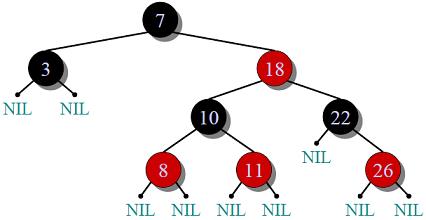
\includegraphics[scale=0.5]{rbt}
  \centering
  \caption{Example of a red-black tree.}
  \label{fig:rbt}
\end{figure}

Every red-black tree satisfy the following two balance invariants:

\begin{enumerate}
  \item No red node has a red child. \label{inv1}
  \item Every path from the root to an empty node contains the same number of black nodes. \label{inv2}
\end{enumerate}

Taken together, these two invariants guarantee that the longest possible path in a red-black tree, one with alternating black and red nodes, is no more than twice as long as the sorthest possible, one with black nodes only.

\begin{theorem}\label{t:balance}
  The maximum depth of a node in a red-black tree of size $n$ is at most $2\lfloor \log (n+1) \rfloor$
\end{theorem}

\begin{proof}\label{p:balance}
  The maximum number of black nodes in the longest path from the root to a leaf is restricted by the number of nodes in the shortest past (inv. \ref{inv2}).

  Assume that the shortest path has depth $k$. Then, there are $k+1$ nodes in a path of depth $k$.

  From the definition of the shortest path, there is a full and complete binary subtree of depth $k$ (that includes the shortest path). Suposse that the complete binary subtree has $n$ nodes. So, by the definition of a complete binary tree, $n = 2^{k+1} -1$. Hence, we can compute the number of nodes in the shortest by using the previous equation.

  \begin{align*}
    n     &= n^{k+1}-1 \\
    k + 1 &= \log_2 (n+1)
  \end{align*}

  The number f nodes in the shortest path is $\log_2 (n+1)$. So, the largest path can have, at most, $\log_2 (n+1)$ black nodes (inv. \ref{inv2}).

  Let's make the largest path with $\log_2 (n+1)$ black nodes. We want to put as many red nodes as possible because we are limited in the number of black nodes. But, because of the inv. \ref{inv1}, we need to alternate between black and red nodes.

  If the root is black, there will be as many red nodes as black ones. The depth $k$ of the largest path is the following:

  \begin{align*}
    k &= \#red \cdot \#black \\
    k &= \log_2 (n+1) \cdot \log_2 (n+1) \\
    k &= 2[ \log_2 (n+1) ] \\
    k &= \mathcal{O}(\log n)
  \end{align*}

\end{proof}

\section{Implementation}\label{s:implementation}

Explain haskell implementation.

\section{Experimentation}\label{s:experimentation}

Design an experiment to show the self-balancing of the structure.

Show that for any input list, the maximum depth of the tree is 2[log (n + 1)]

\section{Conclusion}\label{s:conclusion}

One of the reasons this implementation is so much  simpler than typical presentations of red-black trees (e.g., Chapter 14 of \cite{clr90}) is that it uses subtly different  rebalancing  transformations.  Imperative implementations typically split the four dangerous cases considered here into eight cases, according to the color  of the sibling  of the red node with a red child.  Knowing the color of the red parent's  sibling allows the transformations  to use fewer  assignments in some cases and to terminate rebalancing early in others.

However, in a functional setting, where we are copying the nodes in question  anyway, we cannot reduce the number  of assignments in this fashion, nor can we terminate copying early, so there is no point is using the more complicated transformations.

%%%%%%%%%%%%%%%% BIBLIOGRAPHY %%%%%%%%%%%%%%%%%%%%%

\bibliographystyle{alpha}
\bibliography{refs}

\end{document}
